\documentclass[leqno]{article}
% Shared QBT/Soln pack preamble for resources.danieljsmith.org.
\usepackage{graphicx}
\usepackage{dsfont}
\usepackage{mathtools}
\usepackage{amssymb}
\usepackage{amsmath}
\usepackage{mleftright}
\usepackage{amsthm}
\usepackage{float}
\usepackage{ragged2e}
\usepackage{tensor}
\usepackage{fancyhdr}
\usepackage{empheq}
\usepackage[most]{tcolorbox}
\usepackage{enumitem}
\usepackage{dirtytalk}
\usepackage{marginnote}
\usepackage{microtype}
\usepackage[
  a4paper,
  left=0.8in,
  right=1in,
  top=1in,
  bottom=0.5in,
  headheight=14pt,
  headsep=0.4in
]{geometry}
\setlength{\parindent}{0cm}

% TikZ / PGFPlots
\usepackage{pgfplots}
\pgfplotsset{compat=1.18}
\usepgfplotslibrary{fillbetween, polar}
\usetikzlibrary{calc, positioning}
\usetikzlibrary{angles, quotes}
\usetikzlibrary{arrows.meta}
\usetikzlibrary{decorations.pathreplacing, decorations.markings}
\usetikzlibrary{patterns}
\usetikzlibrary{intersections}

% Links and contents. The contents follow the TMUA papers: compact entries,
% no dot leaders, and each question's mark total in grey after its label.
\usepackage{tocloft}
\tocloftpagestyle{fancy}
\setlength{\cftbeforesubsecskip}{2pt}
\setlength{\cftsubsecindent}{1.5em}
\setlength{\cftsubsecnumwidth}{0pt}
\renewcommand{\cftsubsecfont}{\small\color{black}}
\renewcommand{\cftsubsecpagefont}{\small\color{black}}
\renewcommand{\cftsubsecleader}{\hfill}
\usepackage[colorlinks=true,linkcolor=black,citecolor=magenta,urlcolor=black]{hyperref}%
\urlstyle{same}

% Pack macros
% \marks also adds its value to the current question's total in the .aux
% file, so the contents show each total from the second pass. The write
% happens at shipout, so a box typeset more than once counts once. The
% pack's mark total for the contents-page title is summed the same way.
\makeatletter
\newcount\djs@totalmarks
\newcommand{\djsAddMarks}[2]{%
  \global\advance\djs@totalmarks#2\relax
  \@ifundefined{djs@marks@#1}%
    {\expandafter\xdef\csname djs@marks@#1\endcsname{#2}}%
    {\expandafter\xdef\csname djs@marks@#1\endcsname
      {\the\numexpr\csname djs@marks@#1\endcsname+#2\relax}}}
\RenewDocumentCommand{\marks}{o m}{%
  \protected@write\@auxout{}{\string\djsAddMarks{\number\value{enumi}}{#2}}%
  \IfValueTF{#1}%
    {\marginnote{\raggedright\textbf{[#2]}}[#1]}%
    {\marginnote{\raggedright\textbf{[#2]}}}%
}
\makeatother

\newcommand{\vspacerule}[2]{%
  \par\vspace*{#1}%
  \noindent\hrulefill\par
  \vspace*{#2}%
}

\definecolor{scarlet}{RGB}{205, 40, 75}
% Site colours for the contents-page title: the accent, the rule colour, a
% stronger rule colour for the path separator, and the muted text colour.
\definecolor{djsBurgundy}{RGB}{118, 59, 67}
\definecolor{djsHairline}{RGB}{216, 213, 205}
\definecolor{djsSlash}{RGB}{170, 166, 158}
\definecolor{djsMuted}{RGB}{96, 101, 106}

% Worked-solution box, adapted from the TMUA worked-solutions box. A white breakable box with a left scarlet rule and no surrounding
% frame or tint. A part that breaks fills the rest of its page, so the rule
% runs to the bottom margin; the unbroken or last part ends in a short
% horizontal foot rule so a solution visibly stops. Unlike the TMUA box there
% is no answer label. The box does not grow to the left, so the rule sits at
% the text edge; growing to the right keeps the usable line width close to the
% old tcolorbox Solution box.
% Spacing inside the box: paragraphs are 6pt apart, so source blank lines show
% (solutions put one after each display and none between a lead-in and its
% display). Every display gets 6pt above and 10pt below, whatever the length
% of its lead-in line; align rows are spread by an 8pt \jot; solution parts
% are 14pt apart and sub-parts 8pt; \left and \right space like ordinary
% brackets (mleftright); no single line is stranded at a page break; and
% neither the Solution label nor the line before a list ends a page. No
% skip can shrink, so full pages are not squeezed.
\newtcolorbox{djsSolution}{%
  enhanced, breakable, frame hidden, sharp corners, colback=white,
  height fixed for=first and middle, height fill,
  extras unbroken and last={natural height},
  borderline west={2.2pt}{0pt}{scarlet},
  left=11pt, right=0pt, top=5pt, bottom=13pt,
  before skip=13pt, after skip=4pt,
  grow to right by=10mm,
  overlay unbroken and last={%
    \fill[scarlet] (frame.south west)
      rectangle ([xshift=3.5cm, yshift=2.2pt]frame.south west);},
  before upper={{\color{scarlet}\bfseries Solution}\par\nobreak\vspace{4pt}%
    \setlength{\parskip}{6pt plus 2pt}%
    \setlength{\abovedisplayskip}{6pt plus 2pt}%
    \setlength{\abovedisplayshortskip}{6pt plus 2pt}%
    \setlength{\belowdisplayskip}{10pt plus 2pt}%
    \setlength{\belowdisplayshortskip}{10pt plus 2pt}%
    \setlength{\jot}{8pt}%
    \setlist{parsep=6pt plus 2pt, topsep=6pt plus 2pt, beginpenalty=10000}%
    \setlist[enumerate,1]{itemsep=14pt plus 2pt}%
    \setlist[enumerate,2]{itemsep=8pt plus 2pt}%
    \mleftright
    \clubpenalty=10000 \widowpenalty=10000 \displaywidowpenalty=10000\relax}}

% Optional smaller figure inside a solution box. \scalebox shrinks node text
% with the drawing. Not applied to existing figures.
\newcommand{\SolnFigureScale}{0.85}
\newsavebox{\djsSolnFigureBox}
\newenvironment{djsSolutionFigure}
  {\par\vspace{4pt}\begin{center}\begin{lrbox}{\djsSolnFigureBox}}
  {\end{lrbox}\scalebox{\SolnFigureScale}{\usebox{\djsSolnFigureBox}}%
   \end{center}\vspace{2pt}\par}

\newcommand{\cxl}[2]{%
  \tikz[baseline=(X.base)]{%
    \node[inner sep=0pt, outer sep=0pt, text=#1] (X) {$#2$};
    \draw[#1, line width=0.4pt] (X.south west)--(X.north east);
  }%
}

% Page-style hook run at the contents page and each question's opening page.
% A no-op for QBT packs; \djsSolnHeader points it at the fancy header.
\newcommand{\djsQuestionPageStyle}{}

% A contents entry: "Question N" in a box wide enough for two digits, so the
% mark totals line up, then the total in grey. Bookmarks keep "Question N".
\makeatletter
\newlength{\djsTocLabelWidth}
\newcommand{\djsTocMarks}[1]{%
  \@ifundefined{djs@marks@#1}{}{%
    {\footnotesize\itshape\color{black!45}%
     \csname djs@marks@#1\endcsname~mark%
     \ifnum\csname djs@marks@#1\endcsname=1 \else s\fi}}}
\newcommand{\djsTocEntry}[1]{%
  \texorpdfstring
    {\settowidth{\djsTocLabelWidth}{Question 00}%
     \makebox[\dimexpr\djsTocLabelWidth+0.9em\relax][l]{Question #1}%
     \djsTocMarks{#1}}%
    {Question #1}}
\makeatother

% The question count for the contents-page title is written to the .aux at
% the end of the document, so it also appears from the second pass.
\newcounter{djsQuestions}
\newcommand{\questionitem}{%
  \djsQuestionPageStyle
  \item\phantomsection
  \stepcounter{djsQuestions}%
  \addcontentsline{toc}{subsection}{\protect\djsTocEntry{\number\value{enumi}}}%
}
\makeatletter
\newcommand{\djsSetQuestionCount}[1]{\gdef\djs@questioncount{#1}}
\AtEndDocument{\immediate\write\@auxout
  {\string\djsSetQuestionCount{\number\value{djsQuestions}}}}
\makeatother

\renewcommand{\contentsname}{Questions}

% \djsPackHeader[<link content tag>]{<left header>}; the tag says which
% document a click on the header link came from.
\newcommand{\djsPackHeader}[2][questions]{%
  \pagestyle{fancy}%
  \fancyhead{}%
  \fancyfoot{}%
  \renewcommand{\headrulewidth}{0.9pt}%
  \lhead{#2}%
  \chead{}%
  \rhead{\href{https://danieljsmith.org/?utm_source=pdf&utm_campaign=further-maths&utm_content=#1}{danieljsmith.org}}%
}

% The header's topic is also the contents-page title, under which a label
% says which booklet this is.
\newcommand{\djsPackTitle}{}
\newcommand{\djsBookletLabel}{}
\newcommand{\djsQbtHeader}[1]{%
  \djsPackHeader{#1}%
  \renewcommand{\djsPackTitle}{#1}%
  \renewcommand{\djsBookletLabel}{Questions by topic}%
}

% The colophon at the foot of page one, independent of the page style: the
% contents-page title's hairline led by a short scarlet rule, then the date on
% the left and a link to the site on the right, all inside the bottom margin.
% Its sizes are fixed, so it matches the TMUA papers' colophon. The document
% supplies the date; recompiling never changes it.
\makeatletter
\newcommand{\djsLastUpdated}[1]{%
  \AtBeginDocument{\AddToHookNext{shipout/foreground}{\djs@colophon{#1}}}}
\newcommand{\djs@colophon}[1]{%
  \put(0.8in,-\dimexpr\paperheight-0.47in\relax){%
    \makebox[0pt][l]{\color{djsHairline}%
      \rule[0.9pt]{\dimexpr\paperwidth-1.8in\relax}{0.6pt}}%
    \makebox[0pt][l]{\color{scarlet}\rule{3.5cm}{2.2pt}}}%
  \put(0.8in,-\dimexpr\paperheight-0.32in\relax){\makebox[0pt][l]{%
    \fontsize{9}{11}\selectfont Last updated #1}}%
  \put(\dimexpr\paperwidth-1in\relax,-\dimexpr\paperheight-0.32in\relax){%
    \makebox[0pt][r]{\fontsize{7}{8.5}\selectfont\color{djsMuted}%
      Latest version at \href{https://resources.danieljsmith.org/}%
        {\color{black}resources.danieljsmith.org}}}}
\makeatother

% Solutions packs show the header only on the contents page and each
% question's opening page, so it never appears part-way through a solution.
% \thispagestyle marks the next page shipped out, which is the question's
% page because every solution question starts after a \newpage.
\newcommand{\djsSolnHeader}[1]{%
  \djsPackHeader[solutions]{\textit{Solutions} - #1}%
  \pagestyle{empty}%
  \renewcommand{\djsQuestionPageStyle}{\thispagestyle{fancy}}%
  \renewcommand{\djsPackTitle}{#1}%
  \renewcommand{\djsBookletLabel}{Worked solutions}%
}

% \djsSitePath{<strand>}{<topic>}, called once after the header, names where
% the pack sits on the site; the contents-page title prints it above the pack
% title, e.g. CORE PURE / FURTHER CALCULUS. Without it the line is left out.
\makeatletter
\newif\ifdjs@sitepath
\newcommand{\djs@strand}{}
\newcommand{\djs@section}{}
\newcommand{\djsSitePath}[2]{%
  \djs@sitepathtrue
  \renewcommand{\djs@strand}{#1}%
  \renewcommand{\djs@section}{#2}%
}
\makeatother

% Further Mechanics packs call \djsMechanicsPack in their preamble, so that
% \djsFrontMatter prints the default value of g above the contents. The box
% keeps its own space above it (before skip is the whole gap below the title,
% not an addition to it). Without the box, \djsGravityNote is just extra space
% before the contents heading, bringing the gap above it close to the gap
% between the box and the heading on Further Mechanics pages.
\newcommand{\djsGravityNote}{\vspace{14pt}}
\newcommand{\djsMechanicsPack}{%
  \renewcommand{\djsGravityNote}{%
    \begin{tcolorbox}[sharp corners, colback=white, colframe=black,
      boxrule=1pt, left=8pt, right=8pt, top=6pt, bottom=6pt,
      before skip=20pt]
    {\bfseries Instructions}\par\vspace{4pt}
    Unless a question states otherwise, take $g = 9.8\,\mathrm{m\,s^{-2}}$
    wherever a numerical value of $g$ is required. Solutions also give final
    answers for $g = 10\,\mathrm{m\,s^{-2}}$ where these differ.
    \end{tcolorbox}%
    \vspace{16pt}}%
}

% Contents-page title: the site path in spaced burgundy capitals, the pack
% title, a hairline led by a short scarlet rule (the solution box's foot rule),
% then the booklet label with the question and mark counts. The counts come
% from the .aux, so they appear from the second pass.
\makeatletter
\newsavebox{\djs@eyebrowbox}
\newcommand{\djs@caps}[1]{\textls[180]{\MakeUppercase{#1}}}
\newcommand{\djs@eyebrow}{%
  \color{djsBurgundy}\footnotesize\bfseries
  \djs@caps{\djs@strand}%
  {\color{djsSlash}\hspace{0.55em}/\hspace{0.55em}}%
  \djs@caps{\djs@section}}
\newcommand{\djs@dot}{\hspace{0.45em}\textperiodcentered\hspace{0.45em}}
\newcommand{\djs@counts}{%
  \@ifundefined{djs@questioncount}{}{%
    \djs@questioncount~question\ifnum\djs@questioncount=1 \else s\fi
    \ifnum\djs@totalmarks>0
      \djs@dot\the\djs@totalmarks~mark\ifnum\djs@totalmarks=1 \else s\fi
    \fi}}
\newcommand{\djsContentsTitle}{%
  \ifdjs@sitepath
    \sbox\djs@eyebrowbox{\djs@eyebrow}%
    \ifdim\wd\djs@eyebrowbox>\linewidth
      \@latex@warning@no@line{The \string\djsSitePath\space line is wider
        than the text, so it wraps. Shorten its topic}%
    \fi
    {\raggedright\djs@eyebrow\par}%
    \vspace{7pt}%
  \fi
  {\raggedright\fontsize{24.88}{28}\selectfont\djsPackTitle\par}%
  \vspace{9pt}%
  \noindent\makebox[0pt][l]{\color{djsHairline}\rule[0.9pt]{\linewidth}{0.6pt}}%
  {\color{scarlet}\rule{3.5cm}{2.2pt}}\par
  \vspace{5pt}%
  {\small\color{djsMuted}\djsBookletLabel\hfill\djs@counts\par}%
  \vspace{8pt}%
}
\makeatother

\newcommand{\djsFrontMatter}{%
  \djsQuestionPageStyle
  \vspace*{6pt}%
  \djsContentsTitle
  \djsGravityNote
  \tableofcontents
  \newpage
}


\djsSolnHeader{Standard Summations}
\djsSitePath{Core Pure}{Miscellaneous Pure}
\djsLastUpdated{26 October 2026}

\begin{document}
\djsFrontMatter
\begin{enumerate}[
  label=\textbf{\arabic*.},
  leftmargin=*,
  topsep=0pt,
  partopsep=0pt,
  parsep=0pt
]

% ---- Question 1 ----
\questionitem
% [Source: _QBT___Solns__Standard_Summations, Q1]

Using the formulae for $\sum_{r=1}^{n} r$ and $\sum_{r=1}^{n} r^2$, show that
\[\sum_{r=5}^{12} (2r-1)(r+3) = 1556\] \marks[-30pt]{4}

\vspace*{10pt}

\begin{djsSolution}
The standard results are
\[
\sum_{r=1}^{n} r=\frac12 n(n+1),\qquad \sum_{r=1}^{n} r^2=\frac16 n(n+1)(2n+1)
\]

Expanding the general term gives
\[
(2r-1)(r+3)=2r^2+6r-r-3=2r^2+5r-3
\]

so
\[
\sum_{r=1}^{n}(2r-1)(r+3)=2\sum_{r=1}^{n} r^2+5\sum_{r=1}^{n} r-3n
\]

The required sum is the sum from \(r=1\) to \(12\) minus the sum from \(r=1\) to \(4\):
\[
\sum_{r=5}^{12}(2r-1)(r+3)=\sum_{r=1}^{12}(2r-1)(r+3)-\sum_{r=1}^{4}(2r-1)(r+3)
\]

For \(n=12\):
\begin{align*}
\sum_{r=1}^{12} r^2&=\frac16\times12\times13\times25=650,\qquad \sum_{r=1}^{12} r=\frac12\times12\times13=78\\
\sum_{r=1}^{12}(2r-1)(r+3)&=2\times650+5\times78-3\times12=1300+390-36=1654
\end{align*}

For \(n=4\):
\begin{align*}
\sum_{r=1}^{4} r^2&=\frac16\times4\times5\times9=30,\qquad \sum_{r=1}^{4} r=\frac12\times4\times5=10\\
\sum_{r=1}^{4}(2r-1)(r+3)&=2\times30+5\times10-3\times4=60+50-12=98
\end{align*}

Therefore
\[
\sum_{r=5}^{12}(2r-1)(r+3)=1654-98=1556
\]

as required.
\end{djsSolution}

\newpage

% ---- Question 2 ----
\questionitem
% [Source: _QBT___Solns__Standard_Summations, Q2]

Using standard summation results, find the exact value of
\[\sum_{r=21}^{60} (3r-1)(r+2)\] \marks[-30pt]{4}

\vspace*{10pt}

\begin{djsSolution}
Expanding the bracket:
\[
(3r-1)(r+2)=3r^2+5r-2
\]

The standard results are
\[
\sum_{r=1}^{n} r=\frac12 n(n+1),\qquad \sum_{r=1}^{n} r^2=\frac16 n(n+1)(2n+1)
\]

and also \(\sum_{r=1}^{n} 1=n\). Hence
\begin{align*}
\sum_{r=1}^{n}(3r-1)(r+2)&=3\sum_{r=1}^{n} r^2+5\sum_{r=1}^{n} r-2\sum_{r=1}^{n} 1\\
&=\frac12 n(n+1)(2n+1)+\frac52 n(n+1)-2n\\
&=\frac12 n(n+1)\left[(2n+1)+5\right]-2n\\
&=n(n+1)(n+3)-2n\\
&=n\left[(n+1)(n+3)-2\right]\\
&=n\left(n^2+4n+1\right)
\end{align*}

The required sum is the sum from \(r=1\) to \(60\) minus the sum from \(r=1\) to \(20\):
\begin{align*}
\sum_{r=21}^{60}(3r-1)(r+2)&=\sum_{r=1}^{60}(3r-1)(r+2)-\sum_{r=1}^{20}(3r-1)(r+2)\\
&=60\left(60^2+4\times60+1\right)-20\left(20^2+4\times20+1\right)\\
&=60\times3841-20\times481\\
&=230\,460-9620\\
&=220\,840
\end{align*}
\end{djsSolution}

\newpage

% ---- Question 3 ----
\questionitem
% [Source: _QBT___Solns__Standard_Summations, Q3]

Using standard summation results, find the exact value of
\[\sum_{r=11}^{40} r(r-3)(r+3)\] \marks[-30pt]{4}

\vspace*{10pt}

\begin{djsSolution}
First expand the general term:
\[
r(r-3)(r+3)=r\left(r^2-9\right)=r^3-9r
\]

The standard results are
\[
\sum_{r=1}^{n} r=\frac12 n(n+1),\qquad \sum_{r=1}^{n} r^3=\frac14 n^2(n+1)^2
\]

so
\begin{align*}
\sum_{r=1}^{n}\left(r^3-9r\right)&=\frac14 n^2(n+1)^2-\frac92 n(n+1)\\
&=\frac14 n(n+1)\left[n(n+1)-18\right]
\end{align*}

The required sum is the sum from \(r=1\) to \(40\) minus the sum from \(r=1\) to \(10\):
\[
\sum_{r=11}^{40}\left(r^3-9r\right)=\sum_{r=1}^{40}\left(r^3-9r\right)-\sum_{r=1}^{10}\left(r^3-9r\right)
\]

With \(n=40\):
\[
\sum_{r=1}^{40}\left(r^3-9r\right)=\frac14\times40\times41\times(1640-18)=410\times1622=665\,020
\]

With \(n=10\):
\[
\sum_{r=1}^{10}\left(r^3-9r\right)=\frac14\times10\times11\times(110-18)=\frac{110}{4}\times92=2530
\]

Therefore
\[
\sum_{r=11}^{40} r(r-3)(r+3)=665\,020-2530=662\,490
\]
\end{djsSolution}

\newpage

% ---- Question 4 ----
\questionitem
% [Source: _QBT___Solns__Standard_Summations, Q4]

The positive integer $k$ is such that
\[\sum_{r=1}^{k} \left(6r^2 - k^2\right) = 205\] \\
Find the value of $k$, showing clearly that there is only one possible value. \marks{4} \\

\vspace*{10pt}

\begin{djsSolution}
The standard result is
\[
\sum_{r=1}^{k} r^2=\frac16 k(k+1)(2k+1)
\]

The term \(k^2\) does not depend on \(r\), so summing it \(k\) times gives \(k\times k^2=k^3\). Hence
\begin{align*}
\sum_{r=1}^{k}\left(6r^2-k^2\right)&=6\times\frac16 k(k+1)(2k+1)-k^3\\
&=k(k+1)(2k+1)-k^3\\
&=2k^3+3k^2+k-k^3\\
&=k^3+3k^2+k
\end{align*}

Setting this equal to \(205\):
\[
k^3+3k^2+k-205=0
\]

When \(k=5\), \(125+75+5-205=0\), so \((k-5)\) is a factor. Factorising:
\[
(k-5)\left(k^2+8k+41\right)=0
\]

For \(k^2+8k+41=0\), the discriminant is
\[
b^2-4ac=8^2-4\times1\times41=64-164=-100<0
\]

so this quadratic has no real roots. Therefore the only real solution is \(k=5\), which is a positive integer, so there is only one possible value:
\[
k=5
\]
\end{djsSolution}

\newpage

% ---- Question 5 ----
\questionitem
% [Source: _QBT___Solns__Standard_Summations, Q5]

\begin{enumerate}[label=\textbf{(\alph*)}]
  \item Prove that, for all positive integers $n$,
  \[\sum_{r=1}^{n} (2r-1)^3 = n^2\left(2n^2-1\right)\] \marks[-30pt]{5}
  \item Jo evaluated
  \[\dfrac{1}{n^2}\sum_{r=1}^{n} (2r-1)^3\]
  for $n = 2$, $n = 3$ and $n = 4$, and obtained a prime number each time. Jo then made the statement: \\

  ``For all integers $n \geq 2$,
  \[\dfrac{1}{n^2}\sum_{r=1}^{n} (2r-1)^3\]
  is a prime number.'' \\

  Disprove Jo's statement. \marks{2} \\
\end{enumerate}

\vspace*{10pt}

\begin{djsSolution}
\begin{enumerate}[label=\textbf{(\alph*)}, start=1]
  \item The standard results are
\[
\sum_{r=1}^{n} r=\frac12 n(n+1),\qquad \sum_{r=1}^{n} r^2=\frac16 n(n+1)(2n+1),\qquad \sum_{r=1}^{n} r^3=\frac14 n^2(n+1)^2
\]

together with \(\sum_{r=1}^{n} 1 = n\).

Expanding the cubic:
\[
(2r-1)^3 = 8r^3-12r^2+6r-1
\]

So
\begin{align*}
\sum_{r=1}^{n}(2r-1)^3 &= 8\sum_{r=1}^{n} r^3-12\sum_{r=1}^{n} r^2+6\sum_{r=1}^{n} r-\sum_{r=1}^{n} 1\\
&= 8\times\frac14 n^2(n+1)^2-12\times\frac16 n(n+1)(2n+1)+6\times\frac12 n(n+1)-n\\
&= 2n^2(n+1)^2-2n(n+1)(2n+1)+3n(n+1)-n\\
&= n\left[2n(n+1)^2-2(n+1)(2n+1)+3(n+1)-1\right]\\
&= n\left[2n^3+4n^2+2n-4n^2-6n-2+3n+3-1\right]\\
&= n\left(2n^3-n\right)\\
&= n^2\left(2n^2-1\right)
\end{align*}

as required.

  \item Using part (a), for \(n\geq 2\):
\[
\frac{1}{n^2}\sum_{r=1}^{n}(2r-1)^3 = 2n^2-1
\]

When \(n=5\):
\[
2\times 5^2-1 = 49 = 7\times 7
\]

Since \(49\) is not prime, \(n=5\) is a counterexample, so Jo's statement is false.
\end{enumerate}
\end{djsSolution}

\newpage

% ---- Question 6 ----
\questionitem
% [Source: _QBT___Solns__Standard_Summations, Q6]

\begin{figure}[H]
    \centering
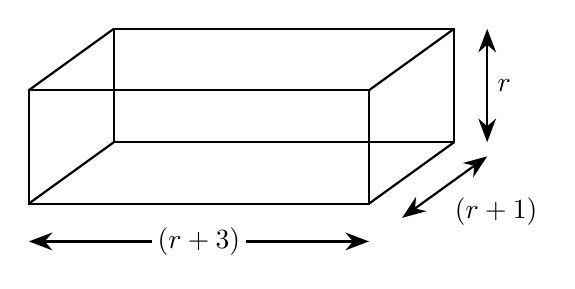
\begin{tikzpicture}[scale=1.2]
\def\L{3.6}
\def\H{1.2}
\def\dx{0.9}
\def\dy{0.65}
\def\off{0.4}
\coordinate (A) at (0,0);
\coordinate (B) at (\L,0);
\coordinate (C) at (\L,\H);
\coordinate (D) at (0,\H);
\foreach \p in {A,B,C,D} { \coordinate (\p2) at ($(\p)+(\dx,\dy)$); }
\draw[thick] (A) -- (B) -- (C) -- (D) -- cycle;
\draw[thick] (A2) -- (B2) -- (C2) -- (D2) -- cycle;
\foreach \p in {A,B,C,D} { \draw[thick] (\p) -- (\p2); }
\draw[{Stealth[length=3mm]}-{Stealth[length=3mm]}, thick] ($(A)+(0,-\off)$) -- ($(B)+(0,-\off)$) node[midway, fill=white, inner sep=2pt] {$(r+3)$};
\draw[{Stealth[length=3mm]}-{Stealth[length=3mm]}, thick] ($(B)+(0.35,-0.15)$) -- ($(B2)+(0.35,-0.15)$) node[midway, below right] {$(r+1)$};
\draw[{Stealth[length=3mm]}-{Stealth[length=3mm]}, thick] ($(B2)+(0.35,0)$) -- ($(C2)+(0.35,0)$) node[midway, right] {$r$};
\end{tikzpicture}
\end{figure}


A block in the shape of a cuboid has length $(r+3)\,\mathrm{cm}$, width $(r+1)\,\mathrm{cm}$ and height $r\,\mathrm{cm}$, as shown in the diagram above. \\

A set consists of $n$ such blocks. The first block has a height of $1\,\mathrm{cm}$, the second block has a height of $2\,\mathrm{cm}$, the third block has a height of $3\,\mathrm{cm}$, and so on, so that the $r$th block has height $r\,\mathrm{cm}$. \\

\begin{enumerate}[label=\textbf{(\alph*)}]
  \item Use the standard results for $\sum_{r=1}^{n} r^3$, $\sum_{r=1}^{n} r^2$ and $\sum_{r=1}^{n} r$ to show that the \textbf{total} volume, $V\,\mathrm{cm}^3$, of all $n$ blocks in the set is given by
  \[V = \dfrac{n}{12}(n+1)(n+2)(3n+13), \qquad n \geq 1\] \marks[-30pt]{5}
  \item Find the smallest number of blocks in the set for which the total volume of the set exceeds $5000\,\mathrm{cm}^3$. \marks{2} \\
\end{enumerate}

\vspace*{10pt}

\begin{djsSolution}
\begin{enumerate}[label=\textbf{(\alph*)}, start=1]
  \item The \(r\)th block has volume
\[
r(r+1)(r+3)=r\left(r^2+4r+3\right)=r^3+4r^2+3r
\]

so the total volume is
\[
V=\sum_{r=1}^{n}\left(r^3+4r^2+3r\right)=\sum_{r=1}^{n}r^3+4\sum_{r=1}^{n}r^2+3\sum_{r=1}^{n}r
\]

The standard results are
\[
\sum_{r=1}^{n} r=\frac12 n(n+1),\qquad \sum_{r=1}^{n} r^2=\frac16 n(n+1)(2n+1),\qquad \sum_{r=1}^{n} r^3=\frac14 n^2(n+1)^2
\]

Substituting these and taking out the common factor \(\frac{n(n+1)}{12}\):
\begin{align*}
V&=\frac14 n^2(n+1)^2+\frac46 n(n+1)(2n+1)+\frac32 n(n+1)\\
&=\dfrac{n(n+1)}{12}\Big[3n(n+1)+8(2n+1)+18\Big]\\
&=\dfrac{n(n+1)}{12}\left(3n^2+3n+16n+8+18\right)\\
&=\dfrac{n(n+1)}{12}\left(3n^2+19n+26\right)
\end{align*}

Factorising the quadratic, \(3n^2+19n+26=(n+2)(3n+13)\), so
\[
V=\dfrac{n}{12}(n+1)(n+2)(3n+13)
\]

as required.

  \item Each block has positive volume, so \(V\) increases as \(n\) increases. Using part (a):
\begin{align*}
n=10:&\quad V=\dfrac{10}{12}\times 11\times 12\times 43=4730<5000\\
n=11:&\quad V=\dfrac{11}{12}\times 12\times 13\times 46=6578>5000
\end{align*}

The smallest number of blocks is \(11\).
\end{enumerate}
\end{djsSolution}

\newpage

% ---- Question 7 ----
\questionitem
% [Source: _QBT___Solns__Standard_Summations, Q7]

\begin{enumerate}[label=\textbf{(\alph*)}]
  \item Use the standard results for $\sum r$, $\sum r^2$ and $\sum r^3$ to show that for all positive integers $n$
  \[\sum_{r=1}^{n} r(2r-1)^2 = \dfrac{1}{6}n(n+1)(an^2+bn+c)\]
  where $a$, $b$ and $c$ are integers to be determined. \marks{5} \\
  \item Hence determine the positive integer $k$ for which
  \[\sum_{r=1}^{k} r(2r-1)^2 = 193\sum_{r=1}^{k} r\] \marks[-30pt]{4}
\end{enumerate}

\vspace*{10pt}

\begin{djsSolution}
\begin{enumerate}[label=\textbf{(\alph*)}, start=1]
  \item First expand the general term:
\[
r(2r-1)^2 = r\left(4r^2-4r+1\right) = 4r^3-4r^2+r
\]

The standard results are
\[
\sum_{r=1}^{n} r=\frac12 n(n+1),\qquad \sum_{r=1}^{n} r^2=\frac16 n(n+1)(2n+1),\qquad \sum_{r=1}^{n} r^3=\frac14 n^2(n+1)^2
\]

So
\begin{align*}
\sum_{r=1}^{n} r(2r-1)^2 &= 4\sum_{r=1}^{n} r^3 - 4\sum_{r=1}^{n} r^2 + \sum_{r=1}^{n} r\\
&= 4\times\frac14 n^2(n+1)^2 - 4\times\frac16 n(n+1)(2n+1) + \frac12 n(n+1)\\
&= n^2(n+1)^2 - \frac23 n(n+1)(2n+1) + \frac12 n(n+1)
\end{align*}

Taking out the common factor \(\frac16 n(n+1)\):
\begin{align*}
\sum_{r=1}^{n} r(2r-1)^2 &= \frac16 n(n+1)\big[6n(n+1) - 4(2n+1) + 3\big]\\
&= \frac16 n(n+1)\left(6n^2+6n-8n-4+3\right)\\
&= \frac16 n(n+1)\left(6n^2-2n-1\right)
\end{align*}

This is in the required form with \(a=6\), \(b=-2\), \(c=-1\).

  \item Using part (a) and the standard result for \(\sum r\), with \(n\) replaced by \(k\), the equation becomes
\[
\frac16 k(k+1)\left(6k^2-2k-1\right) = 193\times\frac12 k(k+1)
\]

Since \(k\) is a positive integer, \(k(k+1)\neq 0\), so dividing both sides by \(\frac16 k(k+1)\) gives
\begin{align*}
6k^2-2k-1 &= 579\\
6k^2-2k-580 &= 0\\
3k^2-k-290 &= 0\\
(k-10)(3k+29) &= 0
\end{align*}

So \(k=10\) or \(k=-\frac{29}{3}\). Since \(k\) is a positive integer, \(k=-\frac{29}{3}\) is rejected, so
\[
k=10
\]

\end{enumerate}
\end{djsSolution}

\newpage

% ---- Question 8 ----
\questionitem
% [Source: _QBT___Solns__Standard_Summations, Q8]

\begin{enumerate}[label=\textbf{(\alph*)}]
  \item Show that
  \[\sum_{r=1}^{n} r^2(r+3)\]
  can be expressed in the form
  \[kn(n+1)(an^2+bn+c)\]
  where $k$ is a rational number and $a$, $b$ and $c$ are integers. \marks{4} \\
  \item Show that there is exactly one positive integer $n$ for which
  \[2\sum_{r=1}^{n} r^2(r+3) = 19\sum_{r=1}^{n} r(r+1)\]
  and state this value of $n$. \marks{6} \\
\end{enumerate}

\vspace*{10pt}

\begin{djsSolution}
\begin{enumerate}[label=\textbf{(\alph*)}, start=1]
  \item Expanding the general term gives \(r^2(r+3)=r^3+3r^2\), so
\[
\sum_{r=1}^{n} r^2(r+3)=\sum_{r=1}^{n} r^3+3\sum_{r=1}^{n} r^2
\]

The standard results are
\[
\sum_{r=1}^{n} r^2=\frac16 n(n+1)(2n+1),\qquad \sum_{r=1}^{n} r^3=\frac14 n^2(n+1)^2
\]

so
\begin{align*}
\sum_{r=1}^{n} r^2(r+3)&=\frac14 n^2(n+1)^2+3\times\frac16 n(n+1)(2n+1)\\
&=\frac14 n^2(n+1)^2+\frac12 n(n+1)(2n+1)\\
&=\frac14 n(n+1)\left[n(n+1)+2(2n+1)\right]\\
&=\frac14 n(n+1)\left(n^2+n+4n+2\right)\\
&=\frac14 n(n+1)\left(n^2+5n+2\right)
\end{align*}

This is in the form \(kn(n+1)(an^2+bn+c)\) with \(k=\frac14\), \(a=1\), \(b=5\), \(c=2\).

  \item First find \(\sum_{r=1}^{n} r(r+1)=\sum_{r=1}^{n} r^2+\sum_{r=1}^{n} r\). The standard result for \(\sum r\) is
\[
\sum_{r=1}^{n} r=\frac12 n(n+1)
\]

and together with the result for \(\sum r^2\) this gives
\begin{align*}
\sum_{r=1}^{n} r(r+1)&=\frac16 n(n+1)(2n+1)+\frac12 n(n+1)\\
&=\frac16 n(n+1)\left[(2n+1)+3\right]\\
&=\frac16 n(n+1)(2n+4)\\
&=\frac13 n(n+1)(n+2)
\end{align*}

Using part (a), the equation becomes
\[
2\times\frac14 n(n+1)\left(n^2+5n+2\right)=19\times\frac13 n(n+1)(n+2)
\]

For a positive integer \(n\), \(n(n+1)\neq 0\), so dividing by \(n(n+1)\) gives
\[
\frac12\left(n^2+5n+2\right)=\frac{19}{3}(n+2)
\]

Multiplying by \(6\):
\begin{align*}
3n^2+15n+6&=38n+76\\
3n^2-23n-70&=0\\
(3n+7)(n-10)&=0
\end{align*}

So \(n=10\) or \(n=-\frac73\). Since \(-\frac73\) is not a positive integer, the only solution that is a positive integer is \(n=10\). Hence there is exactly one positive integer satisfying the equation, namely \(n=10\).
\end{enumerate}
\end{djsSolution}

\newpage

% ---- Question 9 ----
\questionitem
% [Source: _QBT___Solns__Standard_Summations, Q9]

\begin{enumerate}[label=\textbf{(\alph*)}]
  \item Find an expression for
  \[\sum_{r=1}^{2m}(r-1)(r+3)\]
  in the form $\frac{1}{3}m(am^2+bm+c)$, where $a$, $b$, $c$ are integers whose values are to be determined. \marks{4} \\
  \item Hence show that
  \[\sum_{r=2m+1}^{4m}(r-1)(r+3)=\dfrac{1}{3}m\left(56m^2+54m-11\right)\]
  and use this result to find the value of
  \[\sum_{r=21}^{40}(r-1)(r+3)\] \marks[-30pt]{5}
\end{enumerate}

\vspace*{10pt}

\begin{djsSolution}
\begin{enumerate}[label=\textbf{(\alph*)}, start=1]
  \item Expand the general term:
\[
(r-1)(r+3)=r^2+2r-3
\]

The standard results are
\[
\sum_{r=1}^{m} r=\frac12 m(m+1),\qquad \sum_{r=1}^{m} r^2=\frac16 m(m+1)(2m+1)
\]

Using them with \(m\) replaced by \(2m\), together with \(\sum_{r=1}^{2m}3=3\times 2m=6m\), gives
\begin{align*}
\sum_{r=1}^{2m}(r-1)(r+3)&=\sum_{r=1}^{2m}r^2+2\sum_{r=1}^{2m}r-\sum_{r=1}^{2m}3\\
&=\frac16(2m)(2m+1)(4m+1)+2\times\frac12(2m)(2m+1)-6m\\
&=\frac13 m(2m+1)(4m+1)+2m(2m+1)-6m\\
&=\frac13 m\left[(8m^2+6m+1)+6(2m+1)-18\right]\\
&=\frac13 m\left(8m^2+6m+1+12m+6-18\right)\\
&=\frac13 m\left(8m^2+18m-11\right)
\end{align*}

This is in the form \(\frac13 m(am^2+bm+c)\) with \(a=8\), \(b=18\), \(c=-11\).

  \item Replacing \(m\) by \(2m\) in the result of part (a):
\begin{align*}
\sum_{r=1}^{4m}(r-1)(r+3)&=\frac13(2m)\left(8(2m)^2+18(2m)-11\right)\\
&=\frac13(2m)\left(32m^2+36m-11\right)\\
&=\frac13 m\left(64m^2+72m-22\right)
\end{align*}

The required sum is the sum from \(1\) to \(4m\) minus the sum from \(1\) to \(2m\), so
\begin{align*}
\sum_{r=2m+1}^{4m}(r-1)(r+3)&=\sum_{r=1}^{4m}(r-1)(r+3)-\sum_{r=1}^{2m}(r-1)(r+3)\\
&=\frac13 m\left(64m^2+72m-22\right)-\frac13 m\left(8m^2+18m-11\right)\\
&=\frac13 m\left(56m^2+54m-11\right)
\end{align*}

as required.

For \(\sum_{r=21}^{40}(r-1)(r+3)\), take \(2m+1=21\), so \(m=10\), and then \(4m=40\) as needed. Substituting \(m=10\):
\begin{align*}
\sum_{r=21}^{40}(r-1)(r+3)&=\frac13\times 10\left(56\times 100+54\times 10-11\right)\\
&=\frac{10}{3}\times 6129\\
&=20\,430
\end{align*}

\end{enumerate}
\end{djsSolution}

\newpage

% ---- Question 10 ----
\questionitem
% [Source: _QBT___Solns__Standard_Summations, Q10]

\begin{enumerate}[label=\textbf{(\roman*)}]
  \item Use standard series to show that
  \[\sum_{r=1}^{n} r(r+1)(4r-k) = \dfrac{1}{3}n(n+1)(n+2)(3n+1-k)\]
  where $k$ is a constant. \marks{5} \\
  \item Using your result from part (i) with $k=1$, find
  \[\sum_{r=n+1}^{2n} r(r+1)(4r-1)\]
  giving your answer in fully factorised form. \marks{3} \\
\end{enumerate}

\vspace*{10pt}

\begin{djsSolution}
\begin{enumerate}[label=\textbf{(\roman*)}, start=1]
  \item Expanding the general term:
\[
r(r+1)(4r-k)=(r^2+r)(4r-k)=4r^3+(4-k)r^2-kr
\]

The standard results are
\[
\sum_{r=1}^{n} r=\frac12 n(n+1),\qquad \sum_{r=1}^{n} r^2=\frac16 n(n+1)(2n+1),\qquad \sum_{r=1}^{n} r^3=\frac14 n^2(n+1)^2
\]

so
\begin{align*}
\sum_{r=1}^{n} r(r+1)(4r-k)&=4\sum_{r=1}^{n} r^3+(4-k)\sum_{r=1}^{n} r^2-k\sum_{r=1}^{n} r\\
&=n^2(n+1)^2+\frac16(4-k)n(n+1)(2n+1)-\frac12 kn(n+1)\\
&=\frac16 n(n+1)\big[6n(n+1)+(4-k)(2n+1)-3k\big]\\
&=\frac16 n(n+1)\big[6n^2+6n+8n+4-2kn-k-3k\big]\\
&=\frac16 n(n+1)\big[6n^2+14n-2kn+4-4k\big]\\
&=\frac13 n(n+1)\big[3n^2+7n-kn+2-2k\big]
\end{align*}

Expanding gives \((n+2)(3n+1-k)=3n^2+n-kn+6n+2-2k=3n^2+7n-kn+2-2k\), so
\[
\sum_{r=1}^{n} r(r+1)(4r-k)=\dfrac13 n(n+1)(n+2)(3n+1-k)
\]

as required.

  \item Using part (i) with \(k=1\):
\[
\sum_{r=1}^{n} r(r+1)(4r-1)=\dfrac13 n(n+1)(n+2)(3n)=n^2(n+1)(n+2)
\]

Replacing \(n\) by \(2n\):
\[
\sum_{r=1}^{2n} r(r+1)(4r-1)=(2n)^2(2n+1)(2n+2)=8n^2(n+1)(2n+1)
\]

Therefore
\begin{align*}
\sum_{r=n+1}^{2n} r(r+1)(4r-1)&=\sum_{r=1}^{2n} r(r+1)(4r-1)-\sum_{r=1}^{n} r(r+1)(4r-1)\\
&=8n^2(n+1)(2n+1)-n^2(n+1)(n+2)\\
&=n^2(n+1)\big[16n+8-n-2\big]\\
&=n^2(n+1)(15n+6)\\
&=3n^2(n+1)(5n+2)
\end{align*}

\end{enumerate}
\end{djsSolution}

\newpage

% ---- Question 11 ----
\questionitem
% [Source: _QBT___Solns__Standard_Summations, Q11]

\begin{enumerate}[label=\textbf{(\alph*)}]
  \item Use the standard results for $\sum_{r=1}^{n} r^3$, $\sum_{r=1}^{n} r^2$ and $\sum_{r=1}^{n} r$ to show that
  \[\sum_{r=1}^{n} (2r-1)^3 = n^2\left(2n^2 - 1\right)\]
  for all positive integers $n$. \marks{5} \\
  \item Hence find any positive integer values of $n$ for which
  \[\sum_{r=n+1}^{2n} (2r-1)^3 = 29n^4 - 34n^2 + \sum_{r=1}^{\infty} 240\left(\dfrac{3}{5}\right)^{r}\] \marks[-30pt]{5}
\end{enumerate}

\vspace*{10pt}

\begin{djsSolution}
\begin{enumerate}[label=\textbf{(\alph*)}, start=1]
  \item Expanding the cube:
\[
(2r-1)^3=8r^3-12r^2+6r-1
\]

The standard results are
\[
\sum_{r=1}^{n} r=\frac12 n(n+1),\qquad \sum_{r=1}^{n} r^2=\frac16 n(n+1)(2n+1),\qquad \sum_{r=1}^{n} r^3=\frac14 n^2(n+1)^2
\]

and \(\sum_{r=1}^{n} 1=n\). Therefore
\begin{align*}
\sum_{r=1}^{n}(2r-1)^3&=8\sum_{r=1}^{n} r^3-12\sum_{r=1}^{n} r^2+6\sum_{r=1}^{n} r-\sum_{r=1}^{n}1\\
&=8\times\frac14 n^2(n+1)^2-12\times\frac16 n(n+1)(2n+1)+6\times\frac12 n(n+1)-n\\
&=2n^2(n^2+2n+1)-2n(2n^2+3n+1)+3n(n+1)-n\\
&=\left(2n^4+4n^3+2n^2\right)-\left(4n^3+6n^2+2n\right)+\left(3n^2+3n\right)-n\\
&=2n^4-n^2\\
&=n^2\left(2n^2-1\right)
\end{align*}

as required.

  \item Using part (a) with \(n\) replaced by \(2n\):
\[
\sum_{r=1}^{2n}(2r-1)^3=(2n)^2\left(2(2n)^2-1\right)=4n^2\left(8n^2-1\right)=32n^4-4n^2
\]

So the left-hand side is
\begin{align*}
\sum_{r=n+1}^{2n}(2r-1)^3&=\sum_{r=1}^{2n}(2r-1)^3-\sum_{r=1}^{n}(2r-1)^3\\
&=\left(32n^4-4n^2\right)-\left(2n^4-n^2\right)\\
&=30n^4-3n^2
\end{align*}

The infinite series is geometric with first term \(240\times\frac35=144\) and common ratio \(\frac35\). Since \(\left|\frac35\right|<1\), using
\[
S_\infty=\frac{a}{1-r}\qquad(|r|<1)
\]

gives
\[
\sum_{r=1}^{\infty}240\left(\dfrac35\right)^r=\dfrac{144}{1-\frac35}=\dfrac{144}{\frac25}=360
\]

The equation becomes
\begin{align*}
30n^4-3n^2&=29n^4-34n^2+360\\
n^4+31n^2-360&=0\\
\left(n^2+40\right)\left(n^2-9\right)&=0
\end{align*}

Since \(n^2=-40\) has no real solutions, \(n^2=9\). As \(n\) is a positive integer, this gives
\[
n=3
\]

\end{enumerate}
\end{djsSolution}

\newpage

% ---- Question 12 ----
\questionitem
% [Source: _QBT___Solns__Standard_Summations, Q12]

\begin{enumerate}[label=\textbf{(\alph*)}]
  \item Use the standard results for $\sum_{r=1}^{n} r$, $\sum_{r=1}^{n} r^2$ and $\sum_{r=1}^{n} r^3$ to show that, for all positive integers $n$,
  \[\sum_{r=1}^{n} r(r+1)(2r+1) = \dfrac{1}{2}n(n+a)^2(n+b)\]
  where $a$ and $b$ are integers to be found. \marks{5} \\
  \item Given that
  \[\sum_{r=11}^{n} r(r+1)(2r+1) = 17\,940\]
  use your answer to part (a) to find the value of the positive integer $n$, showing clear algebraic working. \marks{4} \\
\end{enumerate}

\vspace*{10pt}

\begin{djsSolution}
\begin{enumerate}[label=\textbf{(\alph*)}, start=1]
  \item Expanding the general term:
\[
r(r+1)(2r+1)=(r^2+r)(2r+1)=2r^3+3r^2+r
\]

The standard results are
\[
\sum_{r=1}^{n} r=\dfrac12 n(n+1),\qquad \sum_{r=1}^{n} r^2=\dfrac16 n(n+1)(2n+1),\qquad \sum_{r=1}^{n} r^3=\dfrac14 n^2(n+1)^2
\]

so
\begin{align*}
\sum_{r=1}^{n} r(r+1)(2r+1)&=2\sum_{r=1}^{n} r^3+3\sum_{r=1}^{n} r^2+\sum_{r=1}^{n} r\\
&=2\times\dfrac14 n^2(n+1)^2+3\times\dfrac16 n(n+1)(2n+1)+\dfrac12 n(n+1)\\
&=\dfrac12 n^2(n+1)^2+\dfrac12 n(n+1)(2n+1)+\dfrac12 n(n+1)\\
&=\dfrac12 n(n+1)\left[n(n+1)+(2n+1)+1\right]\\
&=\dfrac12 n(n+1)\left(n^2+3n+2\right)\\
&=\dfrac12 n(n+1)(n+1)(n+2)\\
&=\dfrac12 n(n+1)^2(n+2)
\end{align*}

This is in the form \(\frac12 n(n+a)^2(n+b)\) with \(a=1\), \(b=2\).

  \item Write \(S_n=\sum_{r=1}^{n} r(r+1)(2r+1)=\frac12 n(n+1)^2(n+2)\). Then
\[
\sum_{r=11}^{n} r(r+1)(2r+1)=S_n-S_{10}
\]

where
\[
S_{10}=\dfrac12\times10\times11^2\times12=7260
\]

Hence
\begin{align*}
\dfrac12 n(n+1)^2(n+2)-7260&=17\,940\\
\dfrac12 n(n+1)^2(n+2)&=25\,200\\
n(n+2)(n+1)^2&=50\,400
\end{align*}

Let \(m=n+1\), so that \(n(n+2)=(m-1)(m+1)=m^2-1\). Then
\begin{align*}
(m^2-1)m^2&=50\,400\\
m^4-m^2-50\,400&=0\\
(m^2-225)(m^2+224)&=0
\end{align*}

Since \(m^2>0\), \(m^2=225\), and as \(n\) is a positive integer, \(m=n+1>0\), so \(m=15\). Therefore
\[
n=14
\]

\end{enumerate}
\end{djsSolution}

\newpage

% ---- Question 13 ----
\questionitem
% [Source: _QBT___Solns__Standard_Summations, Q13]

In this question you may assume the results for
\[\sum_{r=1}^{n} r^3, \quad \sum_{r=1}^{n} r^2 \quad \text{and} \quad \sum_{r=1}^{n} r\] \\
\begin{enumerate}[label=\textbf{(\alph*)}]
  \item Show that
  \[1^3 - 2^3 + 3^3 - 4^3 + \cdots + (2n-1)^3 - (2n)^3 = -n^2(4n+3)\] \marks[-20pt]{5}
\end{enumerate}
Ten consecutive positive integers are written down, the smallest of which is odd. Starting with the cube of the smallest integer, the cubes of these ten integers are alternately added and subtracted, so that the cube of the largest integer is subtracted. The result is $-3725$. \\
\begin{enumerate}[label=\textbf{(\alph*)}, resume]
  \item Use the answer to part (a) to determine the smallest of these ten integers. \marks{4} \\
\end{enumerate}

\vspace*{10pt}

\begin{djsSolution}
\begin{enumerate}[label=\textbf{(\alph*)}, start=1]
  \item The standard results are
\[
\sum_{r=1}^{n} r=\frac12 n(n+1),\qquad \sum_{r=1}^{n} r^2=\frac16 n(n+1)(2n+1)
\]

The terms pair up as an odd cube minus the next even cube, so the left-hand side is
\[
\sum_{r=1}^{n}\left[(2r-1)^3-(2r)^3\right]
\]

Expanding the general term:
\begin{align*}
(2r-1)^3-(2r)^3&=\left(8r^3-12r^2+6r-1\right)-8r^3\\
&=-12r^2+6r-1
\end{align*}

Summing from \(r=1\) to \(n\), with \(\sum_{r=1}^{n} 1=n\):
\begin{align*}
\sum_{r=1}^{n}\left(-12r^2+6r-1\right)&=-12\sum_{r=1}^{n}r^2+6\sum_{r=1}^{n}r-\sum_{r=1}^{n}1\\
&=-12\times\frac16 n(n+1)(2n+1)+6\times\frac12 n(n+1)-n\\
&=-2n(n+1)(2n+1)+3n(n+1)-n\\
&=n\left[-2\left(2n^2+3n+1\right)+3n+3-1\right]\\
&=n\left(-4n^2-6n-2+3n+2\right)\\
&=n\left(-4n^2-3n\right)\\
&=-n^2(4n+3)
\end{align*}

as required.

  \item Let the smallest integer be \(2m+1\), where \(m\) is a non-negative integer. Then the largest is \(2m+10\), and the result is
\begin{align*}
&(2m+1)^3-(2m+2)^3+\cdots+(2m+9)^3-(2m+10)^3\\
&=\left[1^3-2^3+\cdots-(2m+10)^3\right]-\left[1^3-2^3+\cdots-(2m)^3\right]
\end{align*}

Using part (a) with \(n=m+5\) and with \(n=m\):
\begin{align*}
-(m+5)^2(4m+23)+m^2(4m+3)&=-3725\\
-\left(4m^3+63m^2+330m+575\right)+4m^3+3m^2&=-3725\\
-60m^2-330m-575&=-3725\\
60m^2+330m-3150&=0\\
2m^2+11m-105&=0\\
(m-5)(2m+21)&=0
\end{align*}

Since \(m\) must be a non-negative integer, \(m=-\frac{21}{2}\) is rejected, so \(m=5\). The smallest integer is \(2\times5+1=11\).
\end{enumerate}
\end{djsSolution}

\newpage

% ---- Question 14 ----
\questionitem
% [Source: _QBT___Solns__Standard_Summations, Q14]

\begin{enumerate}[label=\textbf{(\alph*)}]
  \item Use the standard summation formulae to show that, for $n \in \mathbb{N}$,
  \[\sum_{r=1}^{n} \left(6r^2 + 2r - 8\right) = an(n-b)(n+c)\]
  where $a$, $b$ and $c$ are positive integers to be determined. \marks{4} \\
  \item Explain why, for $k \in \mathbb{N}$,
  \[\sum_{r=1}^{4k+1} r\sin\left(90r\right)^\circ = 2k+1\] \marks[-30pt]{3}
\end{enumerate}
Using the results from part (a) and part (b) and showing all your working, \\
\begin{enumerate}[label=\textbf{(\alph*)}, resume]
  \item find the value of the integer $n$, where $n \geq 3$, that satisfies
  \[\sum_{r=3}^{n} \left(6r^2 + 2r - 8\right) = 3\left[\sum_{r=3}^{4n+1} r\sin\left(90r\right)^\circ\right]^2\]
  and show that there are no other such values of $n$. \marks{6} \\
\end{enumerate}

\vspace*{10pt}

\begin{djsSolution}
\begin{enumerate}[label=\textbf{(\alph*)}, start=1]
  \item The standard summation formulae are
\[
\sum_{r=1}^{n} r=\frac12 n(n+1),\qquad \sum_{r=1}^{n} r^2=\frac16 n(n+1)(2n+1)
\]

Also \(\sum_{r=1}^{n} 8=8n\). Splitting the sum:
\begin{align*}
\sum_{r=1}^{n}\left(6r^2+2r-8\right)&=6\sum_{r=1}^{n} r^2+2\sum_{r=1}^{n} r-\sum_{r=1}^{n}8\\
&=n(n+1)(2n+1)+n(n+1)-8n\\
&=n\left[(n+1)(2n+1)+(n+1)-8\right]\\
&=n\left[(n+1)(2n+2)-8\right]\\
&=2n\left[(n+1)^2-4\right]
\end{align*}

Using the difference of two squares, \((n+1)^2-4=(n+1-2)(n+1+2)=(n-1)(n+3)\), so
\[
\sum_{r=1}^{n}\left(6r^2+2r-8\right)=2n(n-1)(n+3)
\]

This is in the form \(an(n-b)(n+c)\) with \(a=2\), \(b=1\), \(c=3\).

  \item The values of \(\sin(90r)^\circ\) for \(r=1,2,3,4\) are \(1,0,-1,0\), and since \(\sin\) has period \(360^\circ\), this pattern repeats every four terms. So the sum is
\[
1+0-3+0+5+0-7+0+\cdots
\]

Group the first \(4k\) terms into \(k\) blocks of four, \(r=4m+1,\ldots,4m+4\) for \(m=0,1,\ldots,k-1\). Each block contributes
\[
(4m+1)(1)+(4m+2)(0)+(4m+3)(-1)+(4m+4)(0)=-2
\]

so the sum of the first \(4k\) terms is \(k\times(-2)=-2k\).

The final term has \(r=4k+1\), and \(\sin(360k+90)^\circ=\sin 90^\circ=1\), so it contributes \(4k+1\). Therefore
\[
\sum_{r=1}^{4k+1} r\sin(90r)^\circ=-2k+(4k+1)=2k+1
\]

as required.

  \item For the left-hand side, remove the \(r=1\) and \(r=2\) terms from the result of part (a). When \(r=1\) the term is \(6+2-8=0\), and when \(r=2\) it is \(24+4-8=20\). So
\[
\sum_{r=3}^{n}\left(6r^2+2r-8\right)=2n(n-1)(n+3)-20
\]

For the right-hand side, use part (b) with \(k=n\) and remove the \(r=1\) and \(r=2\) terms, which are \(1\times\sin 90^\circ=1\) and \(2\times\sin180^\circ=0\):
\[
\sum_{r=3}^{4n+1} r\sin(90r)^\circ=(2n+1)-1-0=2n
\]

so the right-hand side is \(3(2n)^2=12n^2\). The equation becomes
\begin{align*}
2n(n-1)(n+3)-20&=12n^2\\
2n\left(n^2+2n-3\right)-20&=12n^2\\
2n^3+4n^2-6n-20&=12n^2\\
2n^3-8n^2-6n-20&=0\\
n^3-4n^2-3n-10&=0
\end{align*}

Trying \(n=5\): \(125-100-15-10=0\), so \((n-5)\) is a factor. Factorising:
\[
(n-5)\left(n^2+n+2\right)=0
\]

For \(n^2+n+2=0\), the discriminant is
\[
b^2-4ac=1^2-4\times1\times2=-7<0
\]

so this quadratic has no real roots. Hence the only solution is \(n=5\), which satisfies \(n\geq3\), and there are no other such values of \(n\).
\end{enumerate}
\end{djsSolution}

\newpage

% ---- Question 15 ----
\questionitem
% [Source: _QBT___Solns__Standard_Summations, Q15]

\begin{enumerate}[label=\textbf{(\alph*)}]
  \item Explain why, for $n \in \mathbb{N}$,
  \[\sum_{r=1}^{2n} (-1)^r f(r) = \sum_{r=1}^{n} \left(f(2r) - f(2r-1)\right)\]
  for any function $f(r)$. \marks{2} \\
  \item Use the result of part (a) and the standard summation formulae to show that, for $n \in \mathbb{N}$,
  \[\sum_{r=1}^{2n} (-1)^r r^2(r+1) = n(n+1)(4n+1)\] \marks[-30pt]{4}
  \item Hence show that, for $n \in \mathbb{N}$,
  \[\sum_{r=1}^{2n} r(r+1)\left((-1)^r r + 3\right) = n(n+1)(12n+5)\] \marks[-30pt]{3}
  \item Hence evaluate
  \[\sum_{r=11}^{41} r(r+1)\left((-1)^r r + 3\right)\] \marks[-30pt]{4}
\end{enumerate}

\vspace*{10pt}

\begin{djsSolution}
\begin{enumerate}[label=\textbf{(\alph*)}, start=1]
  \item When \(r\) is even, \((-1)^r=1\), and when \(r\) is odd, \((-1)^r=-1\). The values \(r=1,2,\ldots,2n\) split into \(n\) consecutive pairs \(r=2k-1\) (odd) and \(r=2k\) (even), for \(k=1,2,\ldots,n\). Each pair contributes
\[
(-1)^{2k-1}f(2k-1)+(-1)^{2k}f(2k)=f(2k)-f(2k-1)
\]

Adding the contributions of all \(n\) pairs, and renaming the index \(k\) as \(r\), gives
\[
\sum_{r=1}^{2n}(-1)^r f(r)=\sum_{r=1}^{n}\left(f(2r)-f(2r-1)\right)
\]

  \item Take \(f(r)=r^2(r+1)=r^3+r^2\). Then
\begin{align*}
f(2r)&=(2r)^3+(2r)^2=8r^3+4r^2\\
f(2r-1)&=(2r-1)^2(2r)=2r\left(4r^2-4r+1\right)=8r^3-8r^2+2r
\end{align*}

so
\[
f(2r)-f(2r-1)=12r^2-2r
\]

The standard summation formulae are
\[
\sum_{r=1}^{n} r=\frac12 n(n+1),\qquad \sum_{r=1}^{n} r^2=\frac16 n(n+1)(2n+1)
\]

Using part (a):
\begin{align*}
\sum_{r=1}^{2n}(-1)^r r^2(r+1)&=\sum_{r=1}^{n}\left(12r^2-2r\right)\\
&=12\times\frac16 n(n+1)(2n+1)-2\times\frac12 n(n+1)\\
&=2n(n+1)(2n+1)-n(n+1)\\
&=n(n+1)\left(4n+2-1\right)\\
&=n(n+1)(4n+1)
\end{align*}

as required.

  \item Expanding the general term:
\[
r(r+1)\left((-1)^r r+3\right)=(-1)^r r^2(r+1)+3\left(r^2+r\right)
\]

Using the standard formulae with \(n\) replaced by \(2n\):
\begin{align*}
3\sum_{r=1}^{2n}\left(r^2+r\right)&=3\left[\frac16(2n)(2n+1)(4n+1)+\frac12(2n)(2n+1)\right]\\
&=n(2n+1)(4n+1)+3n(2n+1)\\
&=n(2n+1)(4n+4)\\
&=4n(n+1)(2n+1)
\end{align*}

Hence, using part (b):
\begin{align*}
\sum_{r=1}^{2n} r(r+1)\left((-1)^r r+3\right)&=n(n+1)(4n+1)+4n(n+1)(2n+1)\\
&=n(n+1)\left(4n+1+8n+4\right)\\
&=n(n+1)(12n+5)
\end{align*}

as required.

  \item Let \(u_r=r(r+1)\left((-1)^r r+3\right)\) and \(S_m=\sum_{r=1}^{m}u_r\). By part (c), \(S_{2n}=n(n+1)(12n+5)\). Since the result of part (c) applies only to an even upper limit, write
\[
\sum_{r=11}^{41}u_r=S_{41}-S_{10}=S_{40}+u_{41}-S_{10}
\]

Using part (c) with \(n=20\) and \(n=5\):
\begin{align*}
S_{40}&=20\times21\times245=102\,900\\
S_{10}&=5\times6\times65=1950
\end{align*}

Since \(41\) is odd, \((-1)^{41}=-1\), so
\[
u_{41}=41\times42\times(-41+3)=41\times42\times(-38)=-65\,436
\]

Therefore
\[
\sum_{r=11}^{41} r(r+1)\left((-1)^r r+3\right)=102\,900-65\,436-1950=35\,514
\]

\end{enumerate}
\end{djsSolution}

\end{enumerate}
\end{document}
